\chapter{Introduction}
\pagenumbering{arabic}

%%%%%%%%%%%%%%%%%%%%%%%%%%%%%%%%%%%%%%%%%%%%%%%%%%%%%%%%%%%%%%%%%%%%%%%%%%%%%%%%%%%%%%%%%%%%%%%%%%%%

The objective of this project was to implement a control system for an existing hexapod-type robot (shown in Figure~\ref{fig:hexapod}) through the use of the Robot Operating System (ROS) \cite{ros_site}. By attempting to implement a number of complex behaviours, such as environment mapping and autonomous navigation, we aimed to evaluate the usefulness of ROS as a framework for rapidly developing these control systems. Specifically, we looked to explore a range of standard and community-provided packages available for use through ROS which provide state-of-the-art functionality, including those that were necessary for this control system.

\begin{figure}[t]
    \centering
    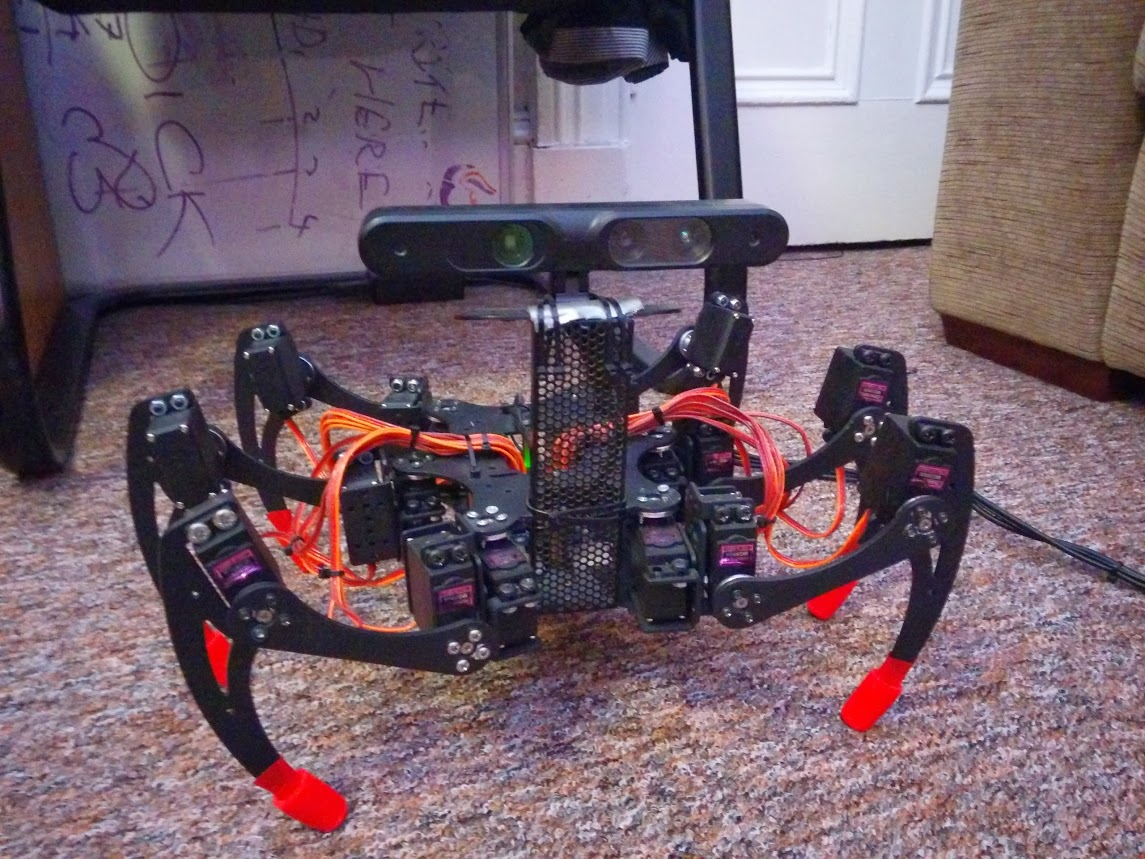
\includegraphics[width=10cm]{hexapod_body1}
    \caption{This hexapod-type which is used as the target hardware platform for this project. The robot has eighteen actuators; three on each limb. A RGB-D camera sits atop as the primary sensor, providing the robot with a 3D view of its immediate environment. A controller sits within the base of the robot, providing the necessary signals to operate the actuators. A bundle of cables protrudes from the back connecting the hardware to a nearby computer for operation, as well as a power source.}
    \label{fig:hexapod}
\end{figure}

This report will detail how this objective was achieved with great success. Through the use of ROS and its packages, it was possible to implement a control system that provides a number of these complex behaviours with relative brevity and simplicity. The resulting robot control system has a number of impressive capabilities:

\begin{description}
	\item[Hardware Interaction] \hfill \\
	The system is capable with interacting with the RGB-D camera and servo controller on-board the robot. Commands can be sent through the system to the controller, allowing for the movement of any particular actuator. Image data from the sensor is received, processed, and then broadcast throughout the system, such that any subsystem needing the imagery can access it.

	\item[Locomotion] \hfill \\
	The system allows the robot to walk with a tripod-type walk gait in an abstracted manner. This abstraction allows any control subsystems to request linear and angular movements, without regard as to the specific actuator commands. The system also provides a means for calibrating the actuators, allowing for movements to be made precisely. Additionally, the robot can be manually controlled via a standard game controller.

	\item[Sensing] \hfill \\
	The system is capable of building a 3D map of the environment around the robot, updating in real-time as the robot moves around. This map is stored in an efficient manner, allowing the system to quickly determine if any obstacles are nearby. Additionally, the system is capable of localising the position of the robot relative to the environment.

	\item[Navigation] \hfill \\
	The system is capable of fully autonomous navigation. Given a target position, the system will determine the most efficient path through the known environment and then supply the appropriate commands to move the robot to that position. Should the robot encounter any new obstacles, the path will be recalculated in real-time to avoid that obstacle.

\end{description}

Without access to the packages available for use through ROS, each of these capabilities would have taken a great number of man hours to develop, test and integrate. 

\section{Motivation}

\section{Overview}